\documentclass[UTF8]{ctexart}
\usepackage{amsmath}
\usepackage{geometry}
\usepackage{graphicx}
\usepackage{gensymb}
\usepackage{wrapfig}
\usepackage{titlesec}
\usepackage{float}
\usepackage{diagbox}
\usepackage{fancyhdr}
\pagestyle{plain}
\geometry{a4paper,scale=0.8}
\CTEXsetup[format+={\raggedright}]{section} 
\title{量统2014-2015郭永期末}
\author{Deschain}
\titlespacing*{\section}
{0pt}{0pt}{0pt}
\titlespacing*{\subsection}
{0pt}{0pt}{0pt}
\titlespacing*{\paragraph}
{0pt}{0pt}{0pt}
\titlespacing*{\subparagraph}
{0pt}{0pt}{0pt}
\titleformat*{\section}{\normalsize}
\begin{document}
\maketitle
\section*{一、(共30分)简要解释以下概念及其物理内涵:(每题10分,只需要选择解答其中3题)。}
(1)区别全同粒子简并及非简并情形的判据及其物理意义。\\
解答:$e^\alpha>>1$是非简并,否则简并。物理意义:非简并时,每个能级上的粒子数远小于它的简并度,或者说,每个量子态的
平均占据数远小于1,泡利原理的限制不起作用。\\
(2)描述晶格比热中的Debye近似和Einstein近似的区别。\\
解答:Einstein:将固体中原子看做$3N$个独立振子,振子频率相同。\\Debye:在Einstein假设之上,增添两个修正:
振子的频率不同;振子有最大频率。\\
(3)Bose-Einstein凝聚的物理意义。\\
解答:当温度从$T_c$开始下降时,基态上的粒子数迅速增加,粒子数$N_0$与总粒子数$N$具有相同的量级。$T=0K$时,
全部粒子都集中在基态上。\\
(4)根据能量均分定理,考虑双原子分子构成的理想气体定容比热在不同温度区间的可能取值。\\
解答:转动特征温度$\theta^r=\frac{h^2}{8\pi^2Ik}$,振动特征温度$\theta^\nu=\frac{h\nu}{k}$\\
$T<<\theta^r$时,$C_V=C_V^t=\frac{3}{2}Nk$\\
$\theta^r<<T<<\theta^\nu$时,$C_V=C_V^t+C_V^r=\frac{5}{2}Nk$\\
$T>>\theta^\nu$时,$C_V=C_V^t+C_V^r+C_V^\nu=\frac{5}{2}Nk+\frac{Nkx^2e^x}{(e^x-1)^2}$,
$x=\frac{\theta^\nu}{T}=\beta h\nu$\\
(5)Maxwell-Boltzmann统计、Bose-Einstein统计与Fermi-Dirac统计基本假设之区别。\\
解答:MB:粒子可区分,一个量子态上可容纳多个粒子。BE:粒子不可区分,一个量子态上可容纳多个粒子。
FD:粒子不可区分,一个量子态上可容纳1个粒子。\\
(6)统计关联对于量子气体压强和内能的影响。\\
\section*{二、(共15分)在一密闭容器内,充满理想气体。现在容器壁上钻一小孔,且小孔足够小,
  对容器内部的热力学平衡不造成影响。容器内分子做无规则热运动,则单位时间从该孔射出的粒子数量
  等于碰撞到小孔处的粒子数量。试求:(a)容器内气体分子的速率分布函数(5分);(b)射出分子束
  中的速率分布函数(5分);(c)射出速流的最概然速率及方均根速率,说明其物理意义(5分)。(积分表附后)}
解答:\\
(a)$f(v)=4\pi(\frac{m}{2\pi kT})^{3/2}e^{-\frac{mv^2}{2kT}}v^2dv$\\
(b)设小孔面积$dA$,其法线方向沿$z$轴。则在$dt$时间内,能漏出的速度为$v$分子在柱体$vcos\theta dtdS$之内。\\
由麦克斯韦速度分布律,$f(v_x,v_y,v_z)=(\frac{m}{2\pi kT})^{3/2}
  e^{-\frac{m(v_x^2+v_y^2+v_z^2)}{2kT}}dv_xdv_ydv_z$\\
又因为$dv_xdv_ydv_z=v^2sin\theta d\theta d\varphi dv$\\
所以漏出的分子$f(v,\theta,\varphi)=(\frac{m}{2\pi kT})^{3/2}e^{-\frac{mv^2}{2kT}}v^3sin\theta cos\theta dv$\\
$f(v)=\int_0^{\frac{\pi}{2}}d\theta\int_0^{2\pi}d\varphi f(v,\theta,\varphi)
  =\frac{m^2}{2(kT)^2}e^{-\frac{mv^2}{2kT}}v^3$\\
(c)最概然速率$v_m=\sqrt{\frac{3kT}{m}}$\\
方均根速率$v_s=\frac{4kT}{m}$
\section*{三、(共20分)考虑一两能级系统(基态无简并,激发态存在2重简并),能级差为$\Delta$。
  (a)分别讨论定域与全同粒子情形下,两个粒子在系统中的所有可能微观状态(10分)。(b)基于比热与
  $\frac{\partial^2lnZ}{\partial\beta^2}$的关系,求出该系统在定域情况下的比热(5分)。
  (c)作图说明比热随温度变化趋势,讨论高、低温极限物理意义(5分)。}
解答:将$\varepsilon_0$记作1,$\varepsilon_1$记作2和3,例如$A_1$说明粒子在$\varepsilon_0$态。\\
(a)定域$(A_1,B_1),(A_1,B_2),(A_1,B_3),(A_2,B_1),(A_2,B_2),(A_2,B_3),(A_3,B_1),(A_3,B_2),(A_3,B_3)$\\
Bose$(A_1,A_1),(A_1,A_2),(A_1,A_3),(A_2,A_3),(A_2,A_2),(A_3,A_3)$\\
Fermi$(A_1,A_2),(A_2,A_3),(A_1,A_3)$\\
(b)
\begin{equation*}
  \begin{aligned}
     & z=e^{-\alpha-\beta\varepsilon_0}+2e^{-\alpha-\beta\varepsilon_1}        \\
     & \overline{E}=-N\frac{\partial lnz}{\partial\beta}
    =N\frac{\varepsilon_0+2\varepsilon_1e^{-\beta\Delta}}{1+2e^{-\beta\Delta}} \\
     & C_v=(\frac{\partial\overline{E}}{\partial T})_V
    =\frac{2N}{kT^2}\frac{\Delta^2e^{-\beta\Delta}}{(1+2e^{-\beta\Delta})^2}
  \end{aligned}
\end{equation*}
(c)
\begin{wrapfigure}{l}{4cm}
  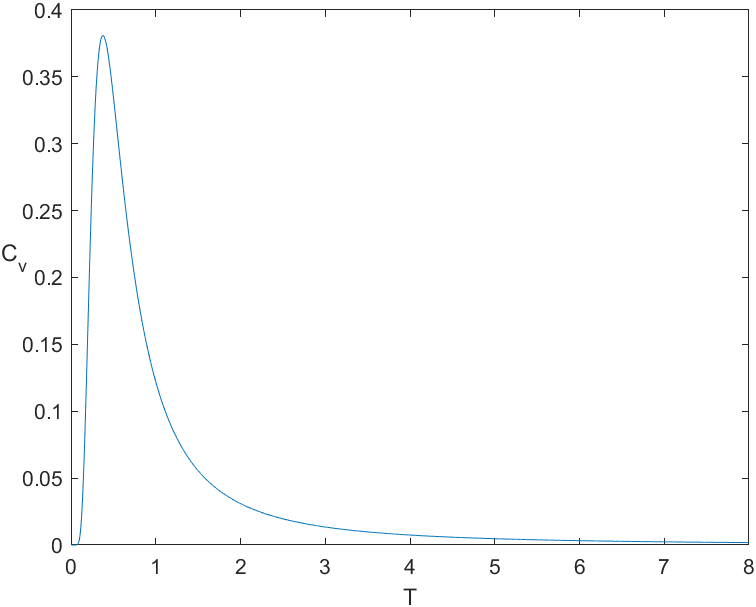
\includegraphics[width=3cm]{3c.png}
\end{wrapfigure}
\newline
低温时,粒子的自由度被冻结;\\
高温时,粒子能级的上升空间很小。\\
\newline\newline
\section*{四、(共15分)电子若在三维的某一维度受到强烈束缚,可形成二维电子气。考虑二维自由电子情况,试求:
  (a)体系的态密度(5分);(b)作图说明绝对零度和$T\neq0$情形,Fermi分布函数随能量的变化关系,并说明其物理意义(5分);
  (c)绝对零度下,体系的Fermi能量和平均能量(5分)。(积分表附后)}
 (a)
\begin{equation*}
  \begin{aligned}
     & \Omega(\varepsilon)=2\pi Sm\varepsilon                      \\
     & g(\varepsilon)d\varepsilon=\frac{1}{h^2}4\pi Smd\varepsilon \\
  \end{aligned}
\end{equation*}
(b)
\subsection*{}
\begin{wrapfigure}{r}{3cm}
  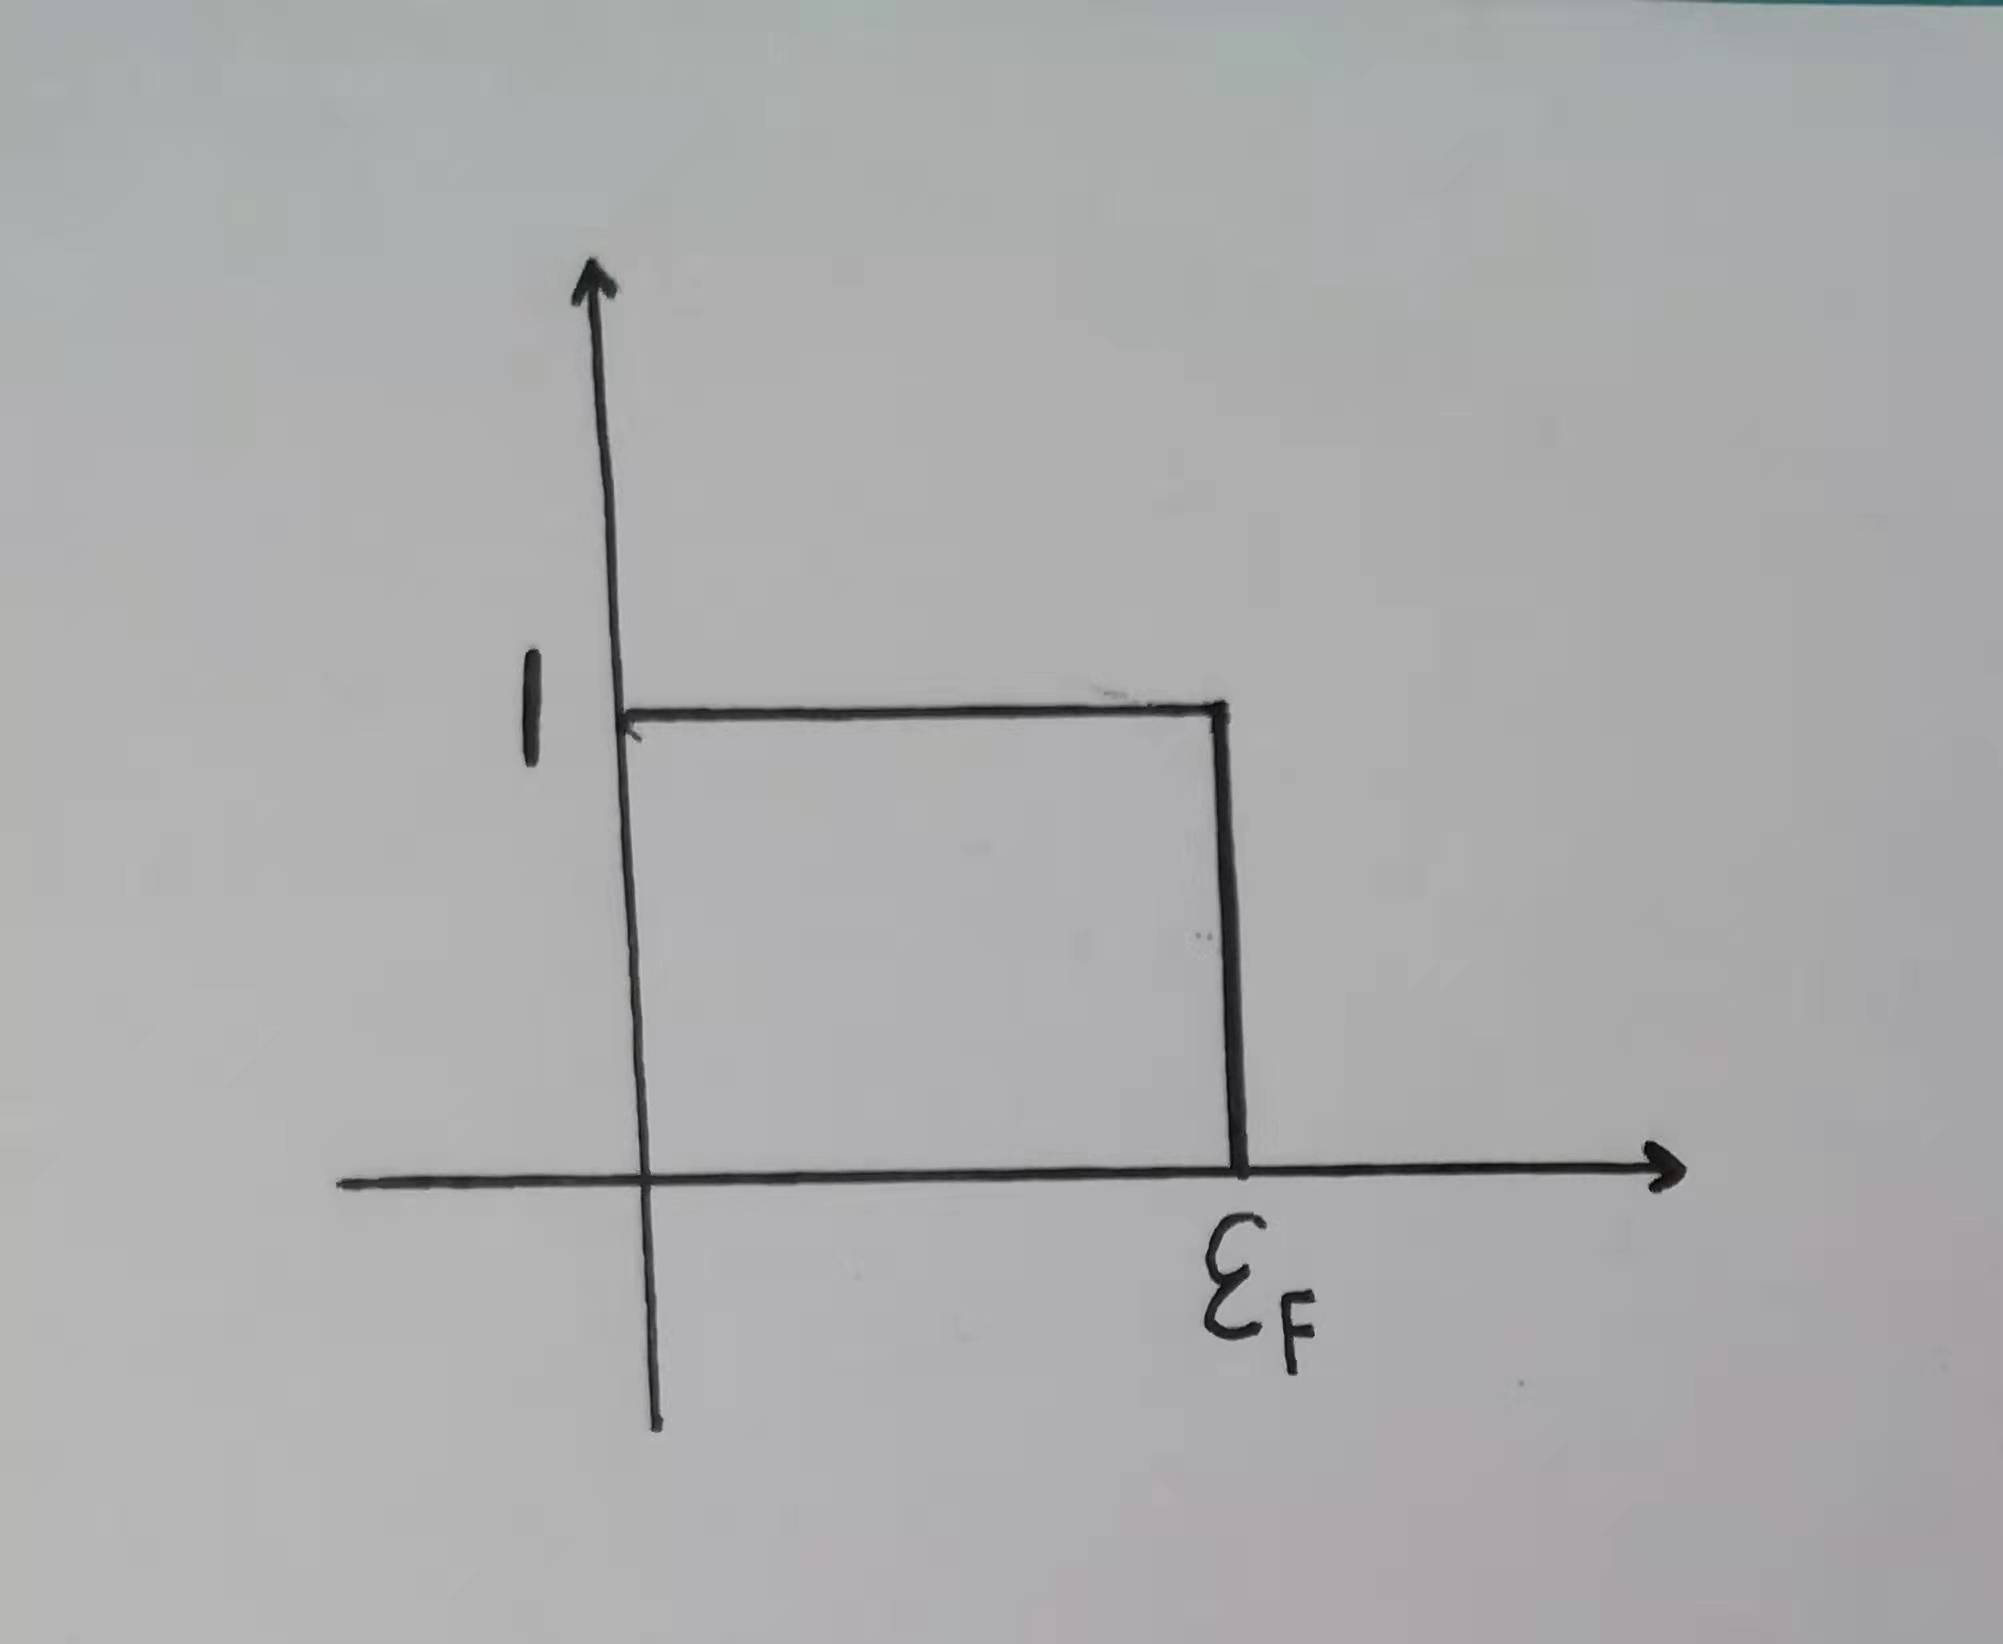
\includegraphics[width=3cm]{4b1.jpg}
\end{wrapfigure}
$T=0K$时,\\
\begin{equation*}
  f(\varepsilon)=\begin{cases}
    1\quad\quad\quad ,\varepsilon<\varepsilon_F \\
    0\quad\quad\quad ,\varepsilon>\varepsilon_F
  \end{cases}
\end{equation*}
绝对零度时,低于$\varepsilon_F$的能级全被填满,高于$\varepsilon_F$的能级则完全空着。
\subsection*{}
\begin{wrapfigure}{r}{3cm}
  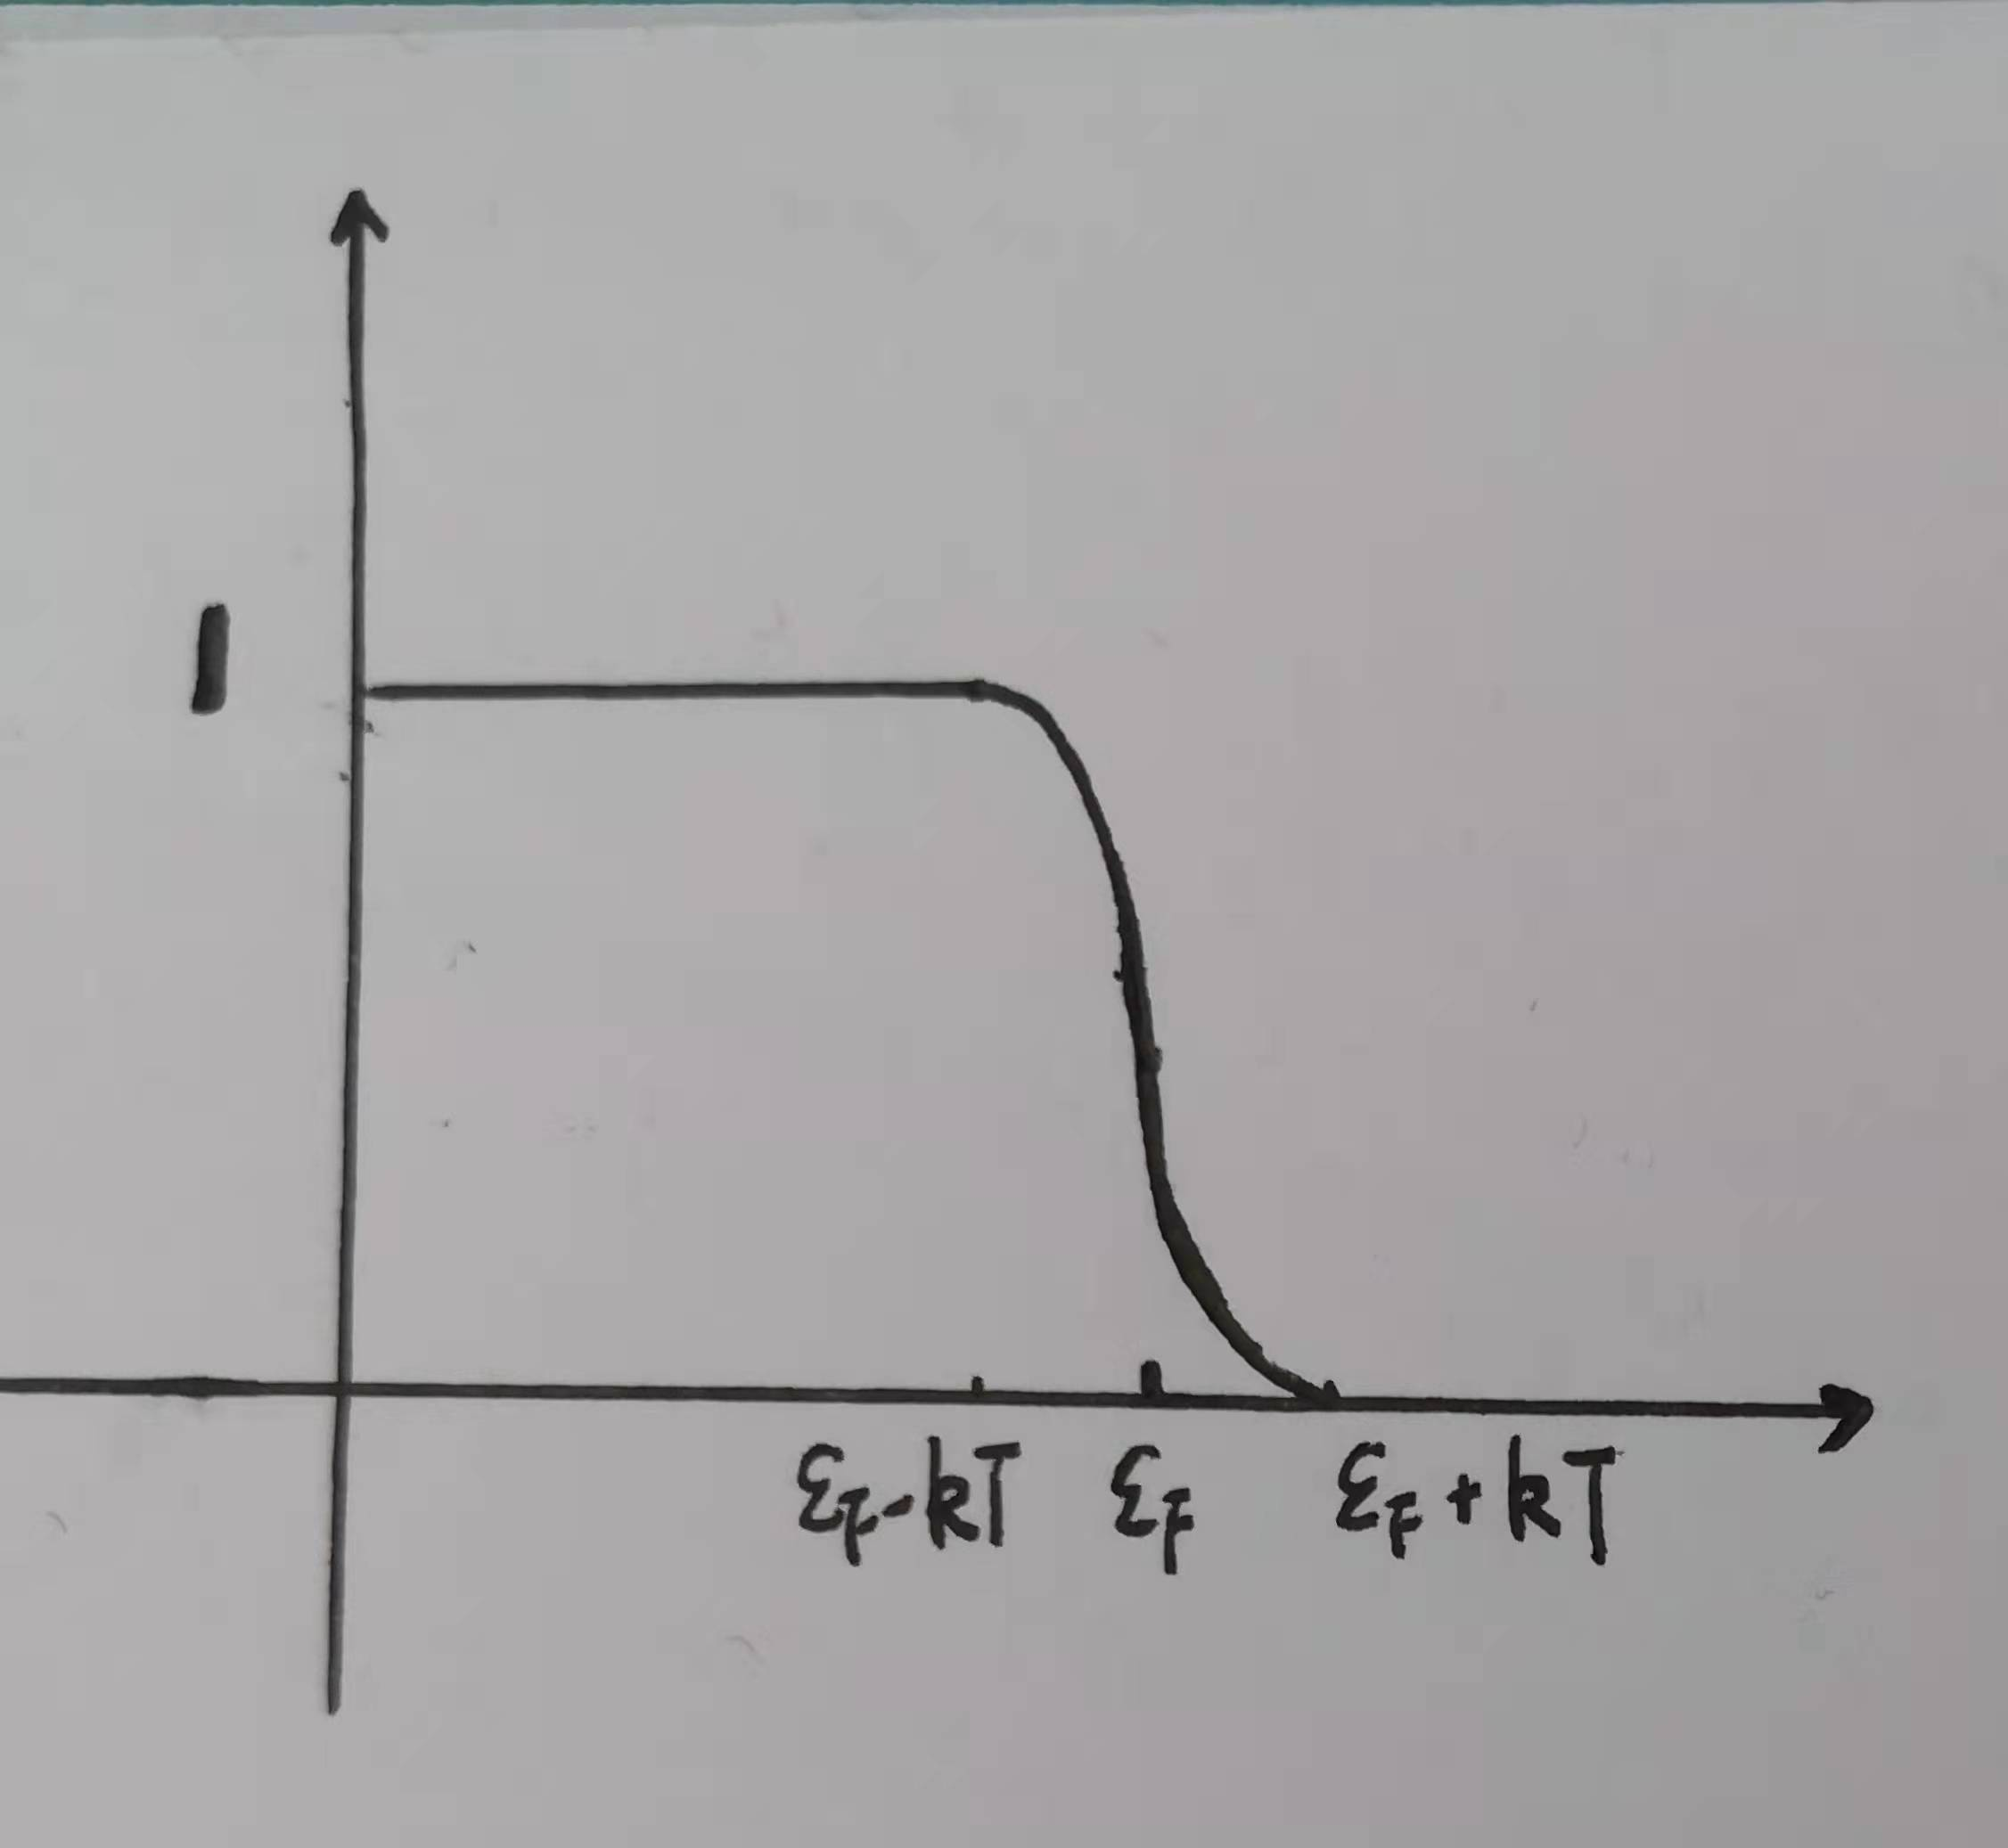
\includegraphics[width=3cm]{4b2.jpg}
\end{wrapfigure}
\begin{equation*}
  f(\varepsilon)=\begin{cases}
    1\quad\quad\quad ,\varepsilon<\varepsilon_F-kT                  \\
    0\sim1\quad\quad ,\varepsilon_F-kT<\varepsilon<\varepsilon_F+kT \\
    0\quad\quad\quad, \varepsilon<\varepsilon_F+kT
  \end{cases}
\end{equation*}
通常$T<<T_F$,粒子分布只在$\varepsilon_F$附近能量宽度为$2kT$的范围内有变化。\\
(c)
\begin{equation*}
  \begin{aligned}
     & N=\int_0^{\varepsilon_F}g(\varepsilon)d\varepsilon
    =\int_0^{\varepsilon_F}\frac{4\pi Sm}{h^2}d\varepsilon
    =\frac{4\pi Sm\varepsilon_F}{h^2}                                            \\
     & \varepsilon_F=\frac{Nh^2}{4\pi Sm}                                        \\
     & \overline{E}=\int_0^{\varepsilon_F}\varepsilon g(\varepsilon)d\varepsilon
    =\frac{2\pi Sm\varepsilon_F^2}{h^2}
    =\frac{N^2h^2}{8\pi Sm}
  \end{aligned}
\end{equation*}
\section*{五、(共20分)依据Plank能量量子化理论,热辐射可以描述为一系列具有量子化能量的简正振动。
  (a)根据Einstein波粒二象性,光可作为粒子处理,其能量、振动频率、动量与光速具有如下关系$E=h\nu=cp$。基于此,
  求不同振动频率$\nu$所对应的态密度(5分);(b)导出热平衡辐射的Plank公式(5分)并求出辐射内能(5分);
  (c)在Plank波动观点中,简正振动模式是可以分辨的,服从Maxwell Boltzmann分布。求频率为$\nu$的这些振子所
  对应的配分函数(5分)。(积分表附后)}
 (a)
\begin{equation*}
  \begin{aligned}
     & g(p)dp=\frac{8\pi V}{h^3}p^2dp         \\
     & g(\nu)d\nu=\frac{8\pi V}{c^3}\nu^2d\nu
  \end{aligned}
\end{equation*}
(b)
\begin{equation*}
  \begin{aligned}
     & n(\nu)d\nu=\frac{g(\nu)d\nu}{e^{-\frac{\varepsilon}{kT}}-1}
    =\frac{8\pi V\nu^2d\nu}{c^3(e^{\frac{h\nu}{kT}}-1)}                              \\
     & \overline{E}=\int_0^\infty\frac{8\pi Vh\nu^3d\nu}{c^3(e^{\frac{h\nu}{kT}}-1)}
    =\frac{8\pi V(kT)^4}{(hc)^3}\int_0^\infty\frac{y^3}{e^y-1}dy=6VT^4               \\
  \end{aligned}
\end{equation*}
(c)
\begin{equation*}
  \begin{aligned}
    z(\nu)=\int_0^\infty g(\nu)e^{-\beta h\nu}d\nu
    =\frac{8\pi V}{c^3}\int_0^\infty\nu^2e^{-\beta h\nu}d\nu
    =\frac{16\pi V}{(\beta hc)^3}
  \end{aligned}
\end{equation*}

\section*{积分表:}
\begin{equation*}
  \begin{aligned}
     & \int_0^\infty x^{2n}e^{-\lambda x^2}dx=\frac{(2n-1)!!}{2^{n+1}}\sqrt{\frac{\pi}{\lambda^{2n+1}}};\quad\quad
    \int_0^\infty x^{2n+1}e^{-\lambda x^2}dx=\frac{n!}{2\lambda^{n+1}};\quad\quad
    \int_0^\infty \frac{x^{1/2}}{e^x-1}dx\approx2.315;\quad\quad                                                   \\                                                   \\
     & \int_0^\infty \frac{x}{e^x-1}dx=\frac{\pi^2}{6};\quad\quad
    \int_0^\infty \frac{x^{3/2}}{e^x-1}dx\approx1.783;\quad\quad
    \int_0^\infty \frac{x^2}{e^x-1}dx\approx2.404;\quad\quad
    \int_0^\infty \frac{x^3}{e^x-1}dx=\frac{\pi^4}{15};\quad\quad                                                  \\
     & \int_0^\infty \frac{x^{1/2}}{e^x+1}dx\approx0.678;\quad\quad
    \int_0^\infty \frac{x}{e^x+1}dx=\frac{\pi^2}{12};\quad\quad
    \int_{+\infty}^{-\infty}\frac{e^x}{(e^x+1)^2}dx=1;\quad\quad
    \int_{+\infty}^{-\infty}\frac{x^2e^x}{(e^x+1)^2}dx=\frac{\pi^2}{3}
  \end{aligned}
\end{equation*}



\end{document}